\documentclass[a4paper]{article}


\usepackage[utf8]{inputenc}
%\usepackage[T1]{fontenc}
\usepackage[francais]{babel}
\usepackage[left=4.2cm,right=4.2cm,top=3cm,bottom=3cm]{geometry}
\usepackage{graphicx,amsmath,amsthm, amssymb,amsfonts,nicefrac}
\usepackage[svgnames,hyperref]{xcolor}
\usepackage[backref=page, colorlinks, linktocpage, citecolor = blue, linkcolor = blue, urlcolor=blue]{hyperref}
\usepackage{enumitem}
\usepackage{caption}
\usepackage{subcaption}
\usepackage{animate}
\usepackage{zref}

\usepackage{listings}
\usepackage{algorithm}
\usepackage{algorithmic}
\usepackage{color}

\usepackage{titlesec}
\setcounter{secnumdepth}{4}

\definecolor{dkgreen}{rgb}{0,0.6,0}
\definecolor{gray}{rgb}{0.5,0.5,0.5}
\definecolor{mauve}{rgb}{0.58,0,0.82}

\lstset{frame=tb,
  language=Python,
  aboveskip=3mm,
  belowskip=3mm,
  showstringspaces=false,
  columns=flexible,
  basicstyle={\small\ttfamily},
  numbers=none,
  numberstyle=\tiny\color{gray},
  keywordstyle=\color{blue},
  commentstyle=\color{dkgreen},
  stringstyle=\color{mauve},
  breaklines=true,
  breakatwhitespace=true,
  tabsize=3
}

%%%%%% Notations
\newcommand{\N}{\ensuremath{\mathbb{N}}}
\newcommand{\Z}{\ensuremath{\mathbb{Z}}}
\newcommand{\Q}{\ensuremath{\mathbb{Q}}}
\newcommand{\R}{\ensuremath{\mathbb{R}}}
\newcommand{\tsp}{{}^t\!}

%%%%Theorems, Lemmes etc
\newtheorem{theorem}{Théorème}[subsection]
\newtheorem{corollary}[theorem]{Corollaire}
\newtheorem{lemma}[theorem]{Lemme}
\newtheorem{proposition}[theorem]{Proposition}
\theoremstyle{definition}
\newtheorem{definition}[theorem]{Définition}
\newtheorem{remark}[theorem]{Remarque}
\newtheorem{example}[theorem]{Exemple}
\renewcommand{\proofname}{Démonstration}
% abstract styling
\renewenvironment{abstract}
{
	\centerline
	{\large \bfseries \scshape Résumé}
	\begin{quote}
	}
	{
	\end{quote}
}

%%% lines
\frenchspacing
\linespread{1.1}

\title{\huge Des casinos à l'intelligence artificielle\\[15pt] \small Travail Encadré de Recherche M1 DS 2021}
\author{Adrien Maitammar \\ Maxime Le Paumier}
%\email{@}


\begin{document}
\maketitle

\vspace{40pt}

\begin{abstract}
Hex est un jeu de plateau a information complète au règles simples mais pouvant présenté une grande complexité. En effet, des stratégies gagnantes sont connus pour le premier joueur pour des plateaux de taille restreinte. Cependant la recherche de telles stratégies devient impraticable à mesure que la taille du plateau augmente. Il est alors question de trouver des stratégies efficaces à défaut de gagnantes. Nous en allons en présenter 3 reposant sur des méthodes de Monte-Carlo et Monte-Carlo avec recherche arborescente. 
\end{abstract}
\newpage

\renewcommand{\contentsname}{Sommaire}
\tableofcontents
 \clearpage
 
 %INTRODUCTION : 
 
\section{Introduction}

\subsection{Règles du jeu}

Hex est un jeu de société pour deux joueurs dont le but est de relier les deux côtés du plateau correspondant à sa couleur par une ligne continue composée de pièces hexagonales. Avec des règles pourtant simples, la complexité de ce jeu est comparable à celle des échecs, dans le sens où les nombres de coups possibles sont comparables. 

\begin{figure}[h]
	\centering
	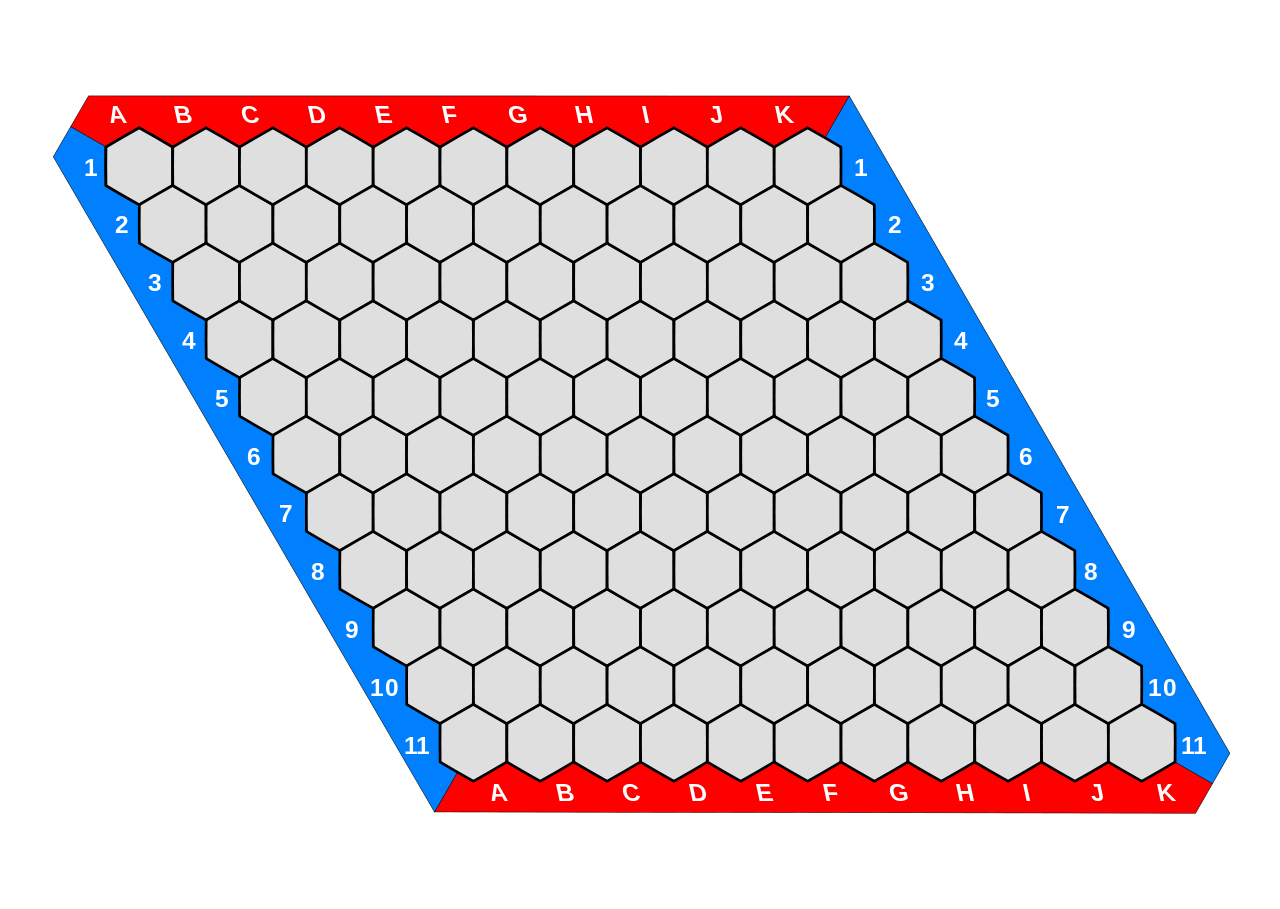
\includegraphics[scale=0.13]{11x11.png}
	\caption{Plateau de jeu 11x11}
\end{figure}

\subsection{Spécificité du jeu}

Une particularité du jeu de Hex est qu'il ne peut pas y avoir de partie aboutissant un match nul. En effet, indépendamment des coups joués et de la taille du plateau, lorsque que le plateau est rempli, il y a obligatoirement un gagnant. Ce résultat a été établit par John Nash et repose sur une preuve par l'absurde.
Ainsi, pour des les plateaux de tailles inférieures ou égales à 9x9 une stratégie gagnante est connu pour le premier joueur. Mais ce n'est pas le cas pour les plateau de taille supérieur et des résultats de la théorie de la complexité montre que la recherche d'une telle stratégie devient très rapidement impraticable quand la taille du jeu augmente. C'est pourquoi, nous allons adopter une approche statistique afin d'obtenir un comportement de jeu optimal de la part d'un joueur programmé avec des techniques d'intelligence artificielle (IA).

\begin{figure}[h]
	\centering
	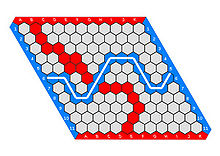
\includegraphics[scale=1]{11x11_gagnant.jpg}
	\caption{Configuration gagnante pour le joueur bleu}
\end{figure}

\section{Implémentation}

\subsection{Python Orienté Objet}

Le jeu a été implémenté en langage Python. Le principaux modules utilisés sont le module pygame pour l'interface graphique pour les parties avec un joueur humain ainsi que le module multiprocessing pour augmenter la rapidité d'exécution des parties dans la phase de test des IA. Le projet est téléchargeable depuis \href{https://github.com/Maxime-LP/Hex-Game}{GitHub}.\\
\\
Concernant la partie orienté objet, nous avons utilisé 3 classes. Une classe principale, \texttt{Game}, faisant interagir deux instances de la classe \texttt{Player} tour par tour en effectuant des actions sur le plateau, instance de la classe \texttt{Board}.

\subsection{Condition de fin de partie}

À chaque coup la fonction fonction \texttt{check\_win} est appelée pour vérifier si la partie a été remporté par un joueur. La rapidité d'exécution de cette fonction a été la principale source d'amélioration qui nous a permis d'augmenter le nombre de parties simulées par seconde. Après une tentative avec la théorie des graphe et l'algorithme de Dijkstra, nous avons opté pour une méthode utilisant les composantes connexes par couleur du plateau. En effet, on considère qu'un joueur gagne s'il relie par une ligne continue les deux bords opposés du plateau, c'est-à-dire si les composantes connexes artificielles Nord et Sud ou Est et Ouest sont des sous ensembles d'une même composante connexe.

\begin{lstlisting}
	def check_win(self, currplayer):
	"""
	Checks if the current player won the game. 
	Returns the winner's name if there is any or None if there is none.
	1 : red player
	2 : blue player
	"""
	
	for component in self.board.components[currplayer.color - 1]:
	if currplayer.color == 1:
	if self.board.north_component.issubset(component) \
	and self.board.south_component.issubset(component):
	return currplayer
	else: # currplayer.color == 2
	if self.board.west_component.issubset(component) \
	and self.board.east_component.issubset(component):
	return currplayer
	return None
\end{lstlisting}

Avec l'utilisation de multiprocessing, nous avons pu atteindre 23000 parties par secondes sur une machine possédant un processeur muni de 48 coeurs.

\newpage


\section{Joueur artificielle}

Au cours du projet, nous avons implémenté des algorithmes de plus en plus performants. Chaque nouvelle version reprenait les bases de la précédente en ajoutant des amélioration, qui nous verrons, au fur et à mesure, se rapproche de la façon dont un joueur humain pourrait jouer et adopte de bons comportements liés à la structure du plateau de jeu.

\subsection{Monte-Carlo}

\subsubsection{Principe}

La première méthode que nous avons programmé est une méthode naïve et empirique. Elle consiste simplement à simuler $n$ de parties réparties équitablement entre les actions possibles pour déterminer le meilleur coup à jouer.

\subsubsection{Algorithme}

\begin{lstlisting}
	def search(self, initialState):
		self.root = treeNode(initialState, None)
		actions = self.root.state.actions
	
		#On copie l'etat actuel du plateau
		for action in actions:
		root_state = deepcopy(self.root.state)
		root_state.takeAction(action, root_state.currplayer)
		node = treeNode(root_state, self.root)
		self.root.children[action] = node
		self.executeRound(node)
		
		#On simule un certain nombre de parties sur chaque action possible
		nb_iter = int(self.searchLimit / len(actions))
		for child in self.root.children.values():
		for i in range(nb_iter):
		self.executeRound(child)
		
		#On selectionne l'action menant au plus haut taux de victoire
		bestChild = self.getBestChild(self.root)
		action = (action for action, node in self.root.children.items() if node is bestChild).__next__()
		
		return action
\end{lstlisting}

Avec cette méthode et en simulant 10000 parties par coups joués, il est possible de voir que le joueur artificielle joue des coups sensés. En effet, il joue majoritairement au centre du plateau, ce qui est une bonne stratégie puisque cela offre davantage de possibilité de connections par la suite.

\newpage 


\subsection{Monte-Carlo et UCB1}

Le problème de l'algorithme Monte-Carlo naïf est qu'il utilise autant de simulation pour chaque coup. De ce fait, il utilise autant de ressources pour évaluer la qualité des mauvais coups que pour évaluer la qualité des bons coups. Le critère de sélection UCB1 permet de pallier à ce problème.
Cet algorithme est nommé \texttt{mc\_ucb1} dans les fichiers Python.

\subsubsection{Principe}

Voici le fonctionnement le l'algorithme: 

\begin{figure}[h]
	\noindent\fbox{%
		\parbox{\textwidth}{%
			\textbf{UCB1} \\
			\textbf{Initialisation:} Jouer chaque coup une fois\\
			\textbf{Boucle:} Jouer le coup $j$ qui maximise $\bar{x_j} + c\sqrt{\frac{\ln{n}}{n_j} }$ avec $\bar{x_j}$ le taux de victoires du coup $j$ jusqu'à présent, $n_j$ le nombre de fois où le coup $j$ a été jouée, $n$ le nombre de coups total joués et $c$ une constante.     
		}%
	}
	\caption{Algorithme UCB1}
\end{figure}

Cette algorithme est initialement conçut pour résoudre le problème du bandit manchot ou, dans sa version générale, du bandit à $K$ bras. Le problème original peut se formuler ainsi : un agent est face à des machines à sous dont il ne connait pas les récompenses moyennes. Son objectif est alors de maximiser ses gains.

Ce problème est en fait un exemple d'apprentissage par renforcement dans lequel l'agent doit faire des compromis entre l'exploitation de la machine qui empiriquement lui rapporte le plus et l'exploration pour espérer trouver une machine rapportant davantage.

L'agent peut bien sûr adopter une approche naïve et jouer la machine maximisant la récompense moyenne sur les coups joués mais  cette stratégie peut le conduire à ignorer certaines machines, qui pourraient être plus intéressantes à jouer. Ansi \\

Peter Auer, Nicol\`o Cesa-Bianchi et Paul Fischer développent dans un article de référence, \textit{Finite-time Analysis of the Multiarmed Bandit Problem}, une stratégie permettant à l'agent de continuer à explorer les machines tout en maximisant ses gains. Plutôt que de procéder naïvement, celui-ci joue les machines selon la procédure UCB1.\\

La constante théorique optimale est $c=\sqrt{2}$. Cependant, bien que des améliorations soit perceptibles, comparé à l'algorithme \texttt{mc}, la constant d'exploration peut être optimiser. Nous reviendrons sur ce point dans la partie concernant l'algorithme UCT. \\ \\
 
Graph mc vs mc\_ucb1.

\subsubsection{Algorithme}

Une notion de nœud est intégrée à l'algorithme. Chaque nœud représente un étant du jeu avec des attributs permettent de calculer son score avec le critère UCB1.
\newpage
\begin{lstlisting}
	class treeNode():
	
		def __init__(self, state, parent):
			self.state = state
			self.parent = parent
			self.numVisits = 0
			self.totalReward = 0
			self.children = {}
			
			# self.root a la couleur du joueur adverse 
			# Les noeuds enfat sont de la couleur du joueur utilisant l'algorithme
			if parent is None : 
				self.player =  3 - state.player
			else:
				self.player = 3 - self.parent.player
\end{lstlisting}

Le nœud \texttt{self.root} représente l'état initial du plateau de jeu, c'est le nœud parent. Il possède ainsi des enfants représentant les coups à évaluer. Compte tenu de ce qui en été dit précédemment, la fonction retournant le meilleurs coup pour l'algorithme \texttt{mc\_ucb1} est la suivante:

\begin{lstlisting}
	def search(self, initialState):
	
		self.root = treeNode(initialState, None)
		actions = self.root.state.actions
		# Initialisation de chaque noeud
		for action in actions:
			root_state = deepcopy(self.root.state)
			root_state.takeAction(action, root_state.currplayer)
			node = treeNode(root_state, self.root)
			self.root.children[action] = node
			self.executeRound(node)
		
		# Simulation avec selection des noeuds via UCB1
		for i in range(self.iterationLimit):
			child = self.selectNode()
			self.executeRound(child)
		
		bestChild = self.ucb1(self.root, 0)
		action = (action for action, node in self.root.children.items() if node is bestChild).__next__()
		return action
	
	def selectNode(self):
		return self.ucb1(self.root, self.explorationConstant)
		
	def ucb1(self, node, explorationValue):
		bestValue = float("-inf")
		bestNodes = []
		for child in node.children.values():
			nodeValue = child.totalReward / child.numVisits + explorationValue * sqrt(log(node.numVisits) / child.numVisits )
			if nodeValue > bestValue:
				bestValue = nodeValue
				bestNodes = [child]
			elif nodeValue == bestValue:
				bestNodes.append(child)
		return random.choice(bestNodes)
\end{lstlisting}

La fonction \texttt{select\_node} calcule le score de chaque nœud via le critère UCB1 renvoyer par la fonction  \texttt{ucb1}. On note qu'une valeur d'exploration nulle correspond au taux de partie gagnées pour un nœud.

\subsection{Upper Confidence bounds applied to Trees (UCT)}

L'algorithme \texttt{mc\_ucb1} permet d'optimiser les simulations sur un coup mais ne permet pas d'anticiper les états du jeu un fois ce coup joué. Il est alors intéressant d'effectuer une recherche arborescente du meilleur coup. Cette méthode est appelée Upper Confidence bounds applied to Trees, nommée \texttt{uct} dans les programmes Python. Cet algorithme de prise de décision est largement développé dans les jeux \footnote{On peut citer son utilisation dans certains programmes de Go, d'Échecs, de Shogi, ou encore le jeu Total War : Rome II}.

\subsubsection{Principe}

On dispose de $n$ simulation par tour.
\begin{figure}[h]
\centering
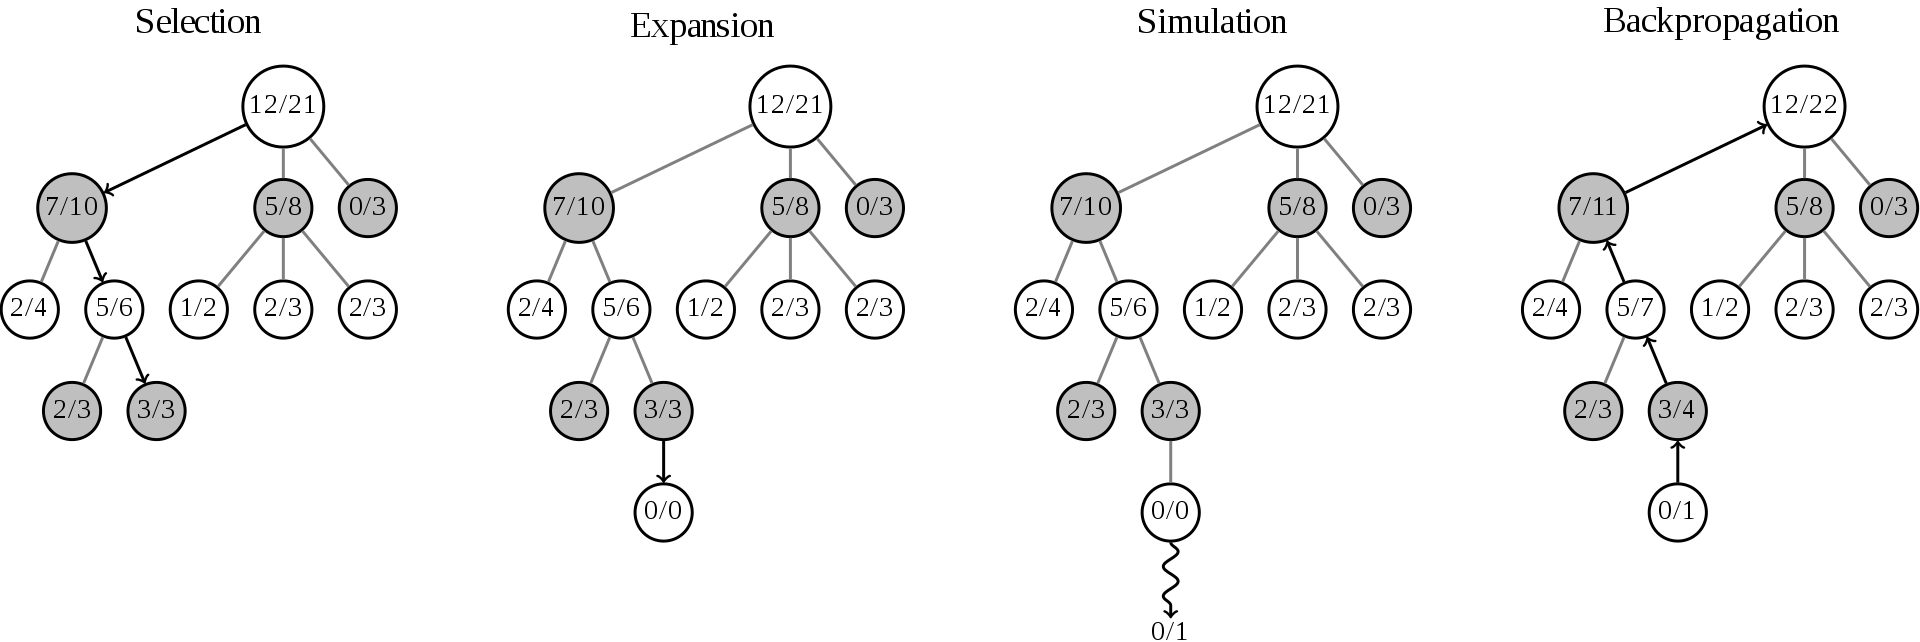
\includegraphics[scale=0.18]{MCTS_wikipedia.png}
\caption{Déroulement d'une simulation avec l'algorithme UCT (\textit{Source : Wikipedia})}
\label{fig:uct}
\end{figure}

Tout d'abord, il faut noter que le coup à la racine de l'arborescence est l'état actuel du plateau. De plus, les nœuds blancs correspondent à un coup joué par le joueur adverse.\\
On initialise tous les nœuds de profondeurs 1 en effectuant une simulation de parties aléatoire sur ces dernier avant de répéter les quatre étapes décrites ci-dessous. La figure 4 est prise comme exemple pour illustrer le propos.\\

1. Sélection\\
Premièrement, on effectue la phase de descente en sélectionnant les nœuds via le critères UCB1 jusqu'à atteindre un nœud sans enfant.\\
Exemple: Les nœuds gris sur la ligne de profondeur 1 ont pour score avec la constance théorique optimale $c=\sqrt{2}$ respectivement de la gauche à la droite $\frac{8}{10} + \sqrt{\frac{2\log21}{10}} \simeq 1,580$, $1.497$ et $1.425$. On choisit donc le nœud de gauche. Puis, on calcule de nouveau les scores des nœuds enfant, ici de profondeur 2. On obtient $1.572$ pour le nœud de gauche et $1.709$ pour le nœud de droite. On sélectionne donc le nœud de droite puis avec le même critère encore le nœud de droite. On arrive à un nœud sans enfant aussi appelé feuille de l'arbre. C'est la fin de la première étape.
\\

2. Expansion\\
Deuxièmement, lorsque on atteint une feuille de l'arbre, on crée un nouveau nœud représentant en nouveau coup joué. Ce coup est choisit de manière aléatoire.\\

3. Simulation\\
Troisièmement, on fini la partie en sélectionnant les coups de manière aléatoire. Dans l'exemple la partie simulée a été perdue.\\

4. Rétro-propagation\\
Quatrièmement, on rétro-propage ce résultat jusqu'à la racine.\\
Exemple: On ajoute 1 au dénominateur (nombre de visites) pour chaque nœuds correspondant aux coups joués et on ajoute 1 au numérateur si la partie simulée a été gagnée et si le nœud est gris, c'est a dire si il correspond a un coup joué par le joueur artificielle utilisant l'algorithme.

Une fois que les $n$ simulations ont été effectuer, sélectionne le nœud de profondeur 1 ayant le meilleur taux de victoire.

\subsubsection{Algorithme}

L'algorithme \texttt{uct} reprend en grande partie de code de l'algorithme \texttt{mc\_ucb1} mais avec une structure d'arbre.

\begin{lstlisting}
	def randomPolicy(state):
		while not state.isTerminal():
			action = random.choice(state.actions)
			state.takeAction(action, state.currplayer)
		return state.getReward()
	
	class treeNode():
		def __init__(self, state, parent):
			self.state = state
			self.parent = parent
			self.numVisits = 0
			self.totalReward = 0
			self.children = {}
			if parent is None : 
				self.player =  3 - state.player
			else:
				self.player = 3 - self.parent.player
	
	def isFullyExpanded(self):
		return len(self.state.actions)==len(self.children)
	
	class UCT():
		def __init__(self, explorationConstant,iterationLimit=None):
			self.iterationLimit = iterationLimit
			self.explorationConstant = explorationConstant
			self.rollout = randomPolicy
		
		def search(self, initialState):
			self.root = treeNode(initialState, None) if root==None else root
			for i in range(self.iterationLimit):
				self.executeRound()
			bestChild = self.getBestChild(self.root, 0)
			action = (action for action, node in self.root.children.items() if node is bestChild).__next__()
			return action
		
		def executeRound(self):
			node = self.selectNode(self.root)
			state = deepcopy(node.state)
			reward = self.rollout(state)
			self.backpropogate(node, reward)
		
		def selectNode(self, node):
			while not node.state.isTerminal():
				if node.isFullyExpanded():
					node = self.getBestChild(node, self.explorationConstant)
				else:
					return self.expand(node)
			return node
		
		def expand(self, node):
			actions = node.state.getPossibleActions()
			while actions!=[]:
				action = random.choice(actions)
				if action not in node.children.keys():
					node_state = deepcopy(node.state)
					node_state.takeAction(action, node_state.currplayer)
					newNode = treeNode(node_state, node)
					node.children[action] = newNode
					return newNode
			
		def backpropogate(self, node, reward):
			while node is not None:
				node.numVisits += 1
				node.totalReward += (reward == 1) * (node.player != self.root.player)
				node = node.parent
		
		def getBestChild(self, node, explorationValue):
			return self.ucb1(node,explorationValue)
		
		def ucb1(self,node,explorationValue):
			bestValue = float("-inf")
			bestNodes = []
			for child in node.children.values():
				nodeValue = child.totalReward / child.numVisits + explorationValue * sqrt(log(node.numVisits) / child.numVisits)
				if nodeValue > bestValue:
					bestValue = nodeValue
					bestNodes = [child]
				elif nodeValue == bestValue:
					bestNodes.append(child)
			return random.choice(bestNodes)
\end{lstlisting}

\subsubsection{Constante d'exploration optimale}

La constante d'exploration optimale ne correspond pas à la valeur théorique $c=\sqrt{2}$. En pratique cette dernière est plus faible pour le jeu de Hex que pour le problème des bandits manchots, les meilleures résultats sont obtenus pour $c \simeq 0.3$. Cette observation semble être partagée pour les jeu ayant des récompense entre 0 et 1, ce qui est le cas ici: une partie gagnée vaut une récompense de 1 et une partie perdue donne une récompense nulle.

\begin{figure}[!h]
	\centering
	\begin{subfigure}{0.32\textwidth}
		\centering
		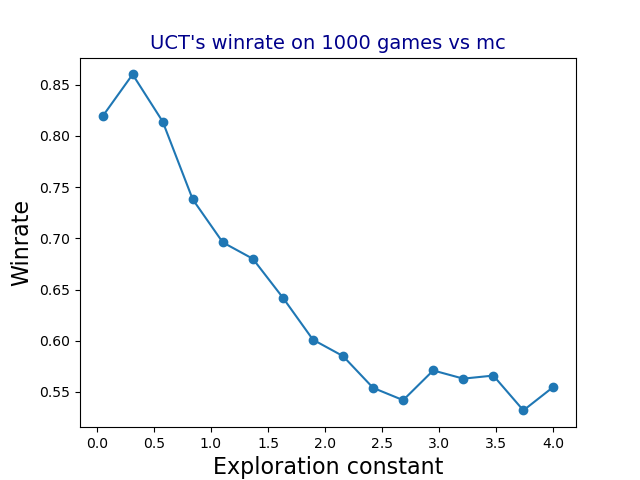
\includegraphics[width=\textwidth]{test1.png}
		\caption{$n=100$, $parties/constante = 2000$, contre \texttt{mc}}
		\label{fig:1_}
	\end{subfigure}
	\hfill
	\begin{subfigure}{0.32\textwidth}
		\centering
		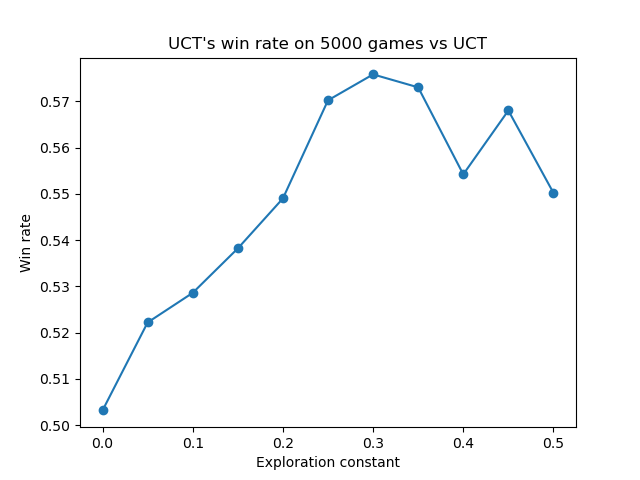
\includegraphics[width=\textwidth]{test2.png}
		\caption{$n=100$, $parties/constante = 2000$, contre \texttt{uct} avec $c = \sqrt{2}$}
		\label{fig:2_}
	\end{subfigure}
	\hfill
	\begin{subfigure}{0.32\textwidth}
		\centering
		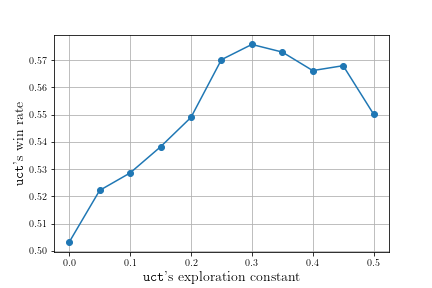
\includegraphics[width=\textwidth]{test3.png}
		\caption{$n=100$, $parties/constante = 5000$, vs \texttt{uct} avec $c = \sqrt{2}$}
		\label{fig:3_}
	\end{subfigure}
	\caption{Constante d'exploration optimal pour UCT}
	\label{fig:best-cst}
\end{figure}

\newpage

\section{Évaluation des algorithmes}


\newpage

\section{Axes d'amélioration}

\subsection{UCT avec mémoire}

L'algorithme \texttt{uct} pourrait garder en mémoire une partie des simulations effectuer pour ses coups suivants. En effet, après avoir joué une première fois, le joueur artificiel \texttt{uct} pourrait tronquer l'arbre et considérer comme racine le nœud correspond à l'état actuel du plateau.\\
\\
Illustration d'arbre tronqué ?\\
\\
Cependant cette méthode ne produit pas  d'amélioration significative si le nombre de simulation par coup n'est pas grand. Car si on tronque l'arbre et en étant optimiste on n'obtient un gain d'informations inférieur à 1\%.

\subsection{Algorithme RAVE et GRAVE}

Un autre axe d'amélioration se trouve en début de partie. Plus il y a de coups possible, moins les estimations de la qualité de ces derniers est juste. C'est pourquoi, compléter l'algorithme \texttt{uct} avec une autre approche serrait intéressant.\\
\\
A développer

\subsection{Connections virtuelles et case mortes}

A développer
\newpage

\section{Conclusion}

A développer

\newpage

\listoffigures 

\newpage

%\bibliographystyle{myalpha}
\begin{thebibliography}{9}

\bibitem{AZ}
Peter Auer, Nicol\`o Cesa-Bianchi \& Paul Fischer, {\em Finite time Analysis of the Multiarmed Bandit Problem}
\bibitem{AZ}
Levente Kocsis \& Csaba Szepesv\`ari, {\em Bandit Based Monte-Carlo Planning}

\end{thebibliography}

\end{document}